% !TeX program = xelatex
% 第三章圖說更新：以每段完整 figure 取代 Overleaf 原本的同名圖。
% 請勿整份 input，避免與正文重複；圖檔與 caption 需一起更新。

% ==================================================
% 位置：3.1.1
% 正文來源：03_01_kinematics.tex
% ==================================================
\begin{figure}[htbp]
    \centering
    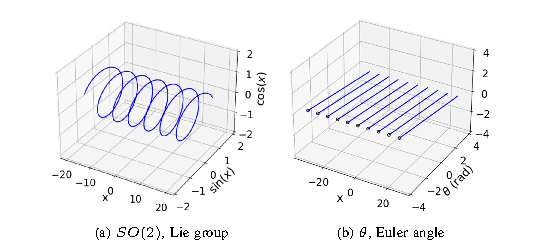
\includegraphics[width=0.95\textwidth]{figsrc/reference_figures/rotation_representation_tang2024.pdf}
    \caption{旋轉群與角度參數表示之比較：(a) $\mathrm{SO}(2)$ 旋轉群表示；(b) 歐拉角參數表示（引自文獻\cite{tang2024gmpc}之圖~1）。}
    \label{fig:ref_rotation_representation}
\end{figure}

% ==================================================
% 位置：3.1.2
% 正文來源：03_01_kinematics.tex
% ==================================================
\begin{figure}[htbp]
    \centering
    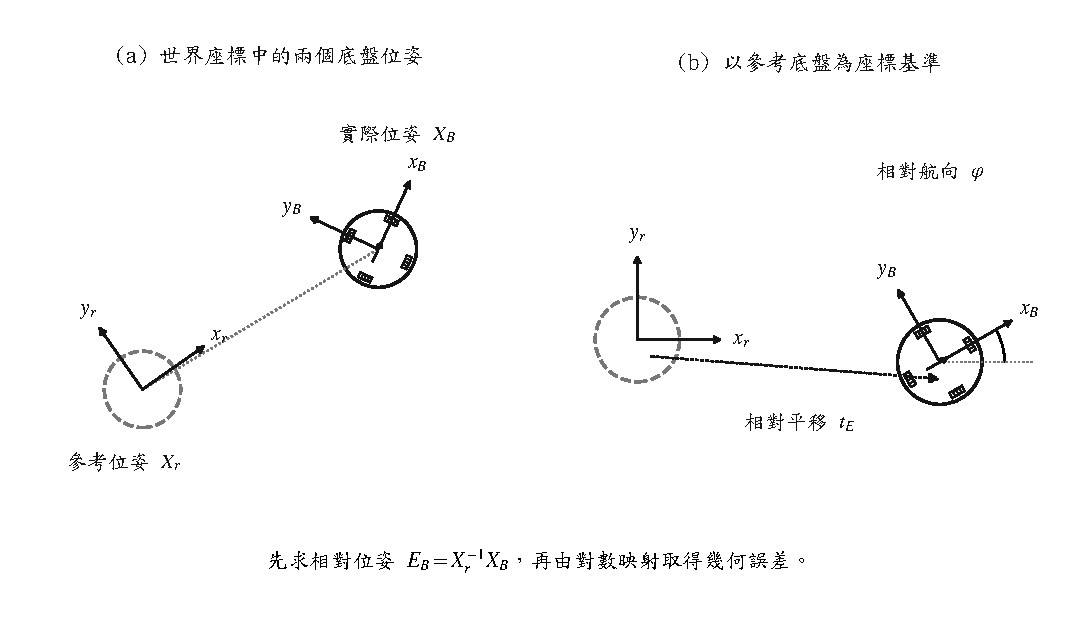
\includegraphics[width=0.98\textwidth]{figsrc/ch03/base_pose_error.pdf}
    \caption{底盤追蹤之相對幾何關係：(a) 世界座標中的參考與實際底盤位姿；(b) 以參考底盤為基準的相對平移與航向。}
    \label{fig:ch3_base_pose_error}
\end{figure}

% ==================================================
% 位置：3.1.3
% 正文來源：03_01_kinematics.tex
% ==================================================
\begin{figure}[htbp]
    \centering
    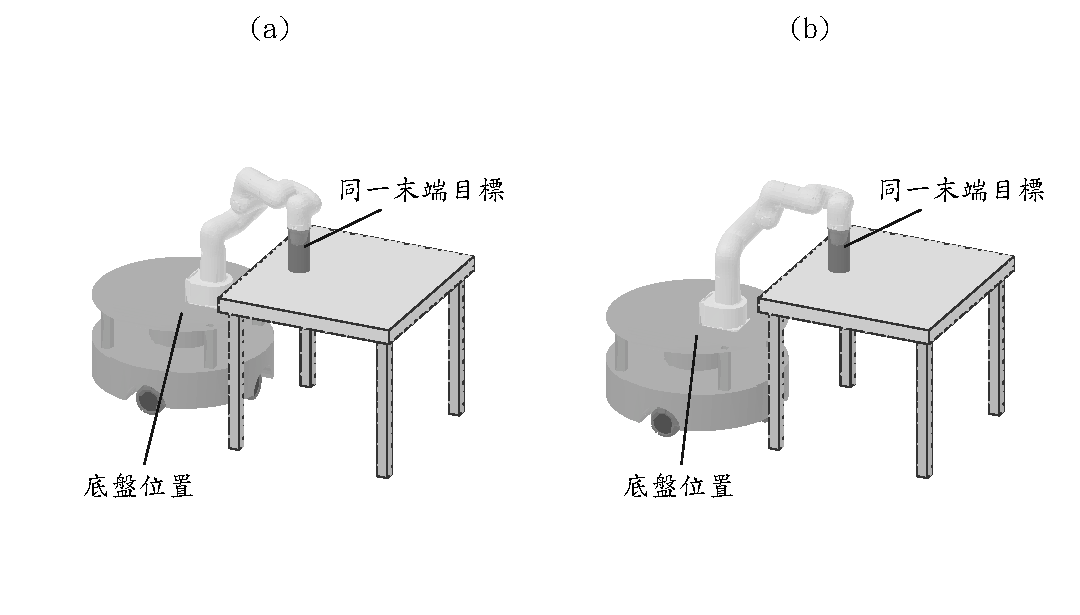
\includegraphics[width=0.98\textwidth]{figsrc/ch03/wholebody_motion_coupling.pdf}
    \caption{底盤側移時之全身運動學耦合：(a) 底盤移動前；(b) 底盤側移後，手臂調整構型以維持相同末端目標。}
    \label{fig:ch3_wholebody_motion_coupling}
\end{figure}

% ==================================================
% 位置：3.2.2
% 正文來源：03_02_augmented_prediction.tex
% ==================================================
\begin{figure}[htbp]
    \centering
    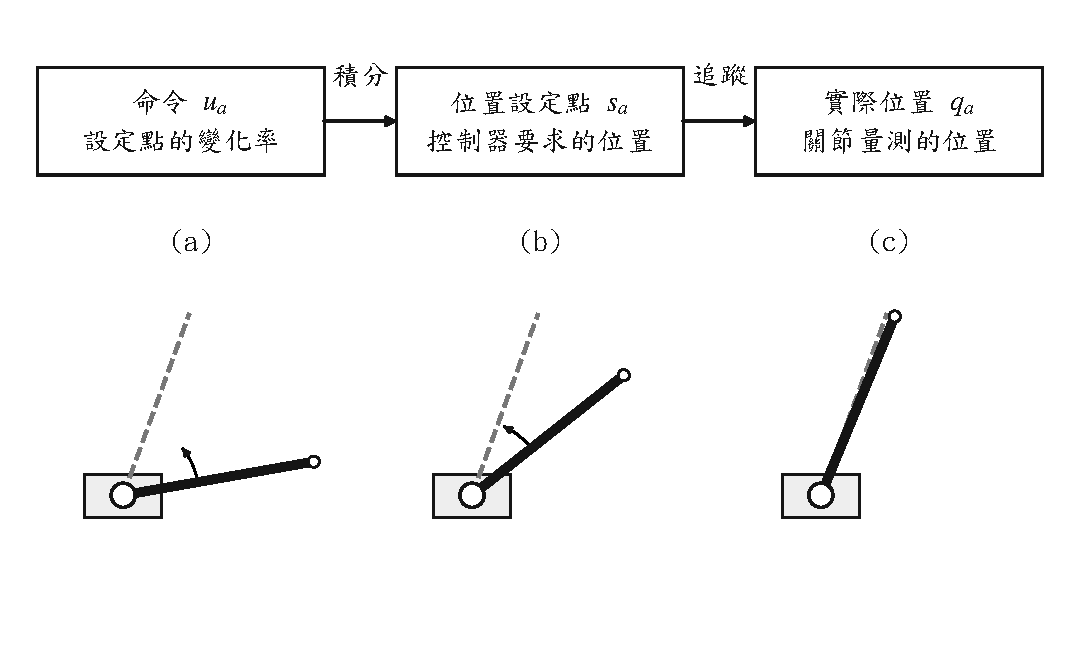
\includegraphics[width=0.98\textwidth]{figsrc/ch03/arm_setpoint_tracking.pdf}
    \caption{手臂設定點與實際關節位置之追蹤關係：(a) 設定點固定；(b) 關節持續追蹤；(c) 關節逐漸接近設定點。虛線與實線分別表示位置設定點與實際關節位置。}
    \label{fig:ch3_arm_setpoint_tracking}
\end{figure}

% ==================================================
% 位置：3.3.2
% 正文來源：03_03_objective_constraints.tex
% ==================================================
\begin{figure}[htbp]
    \centering
    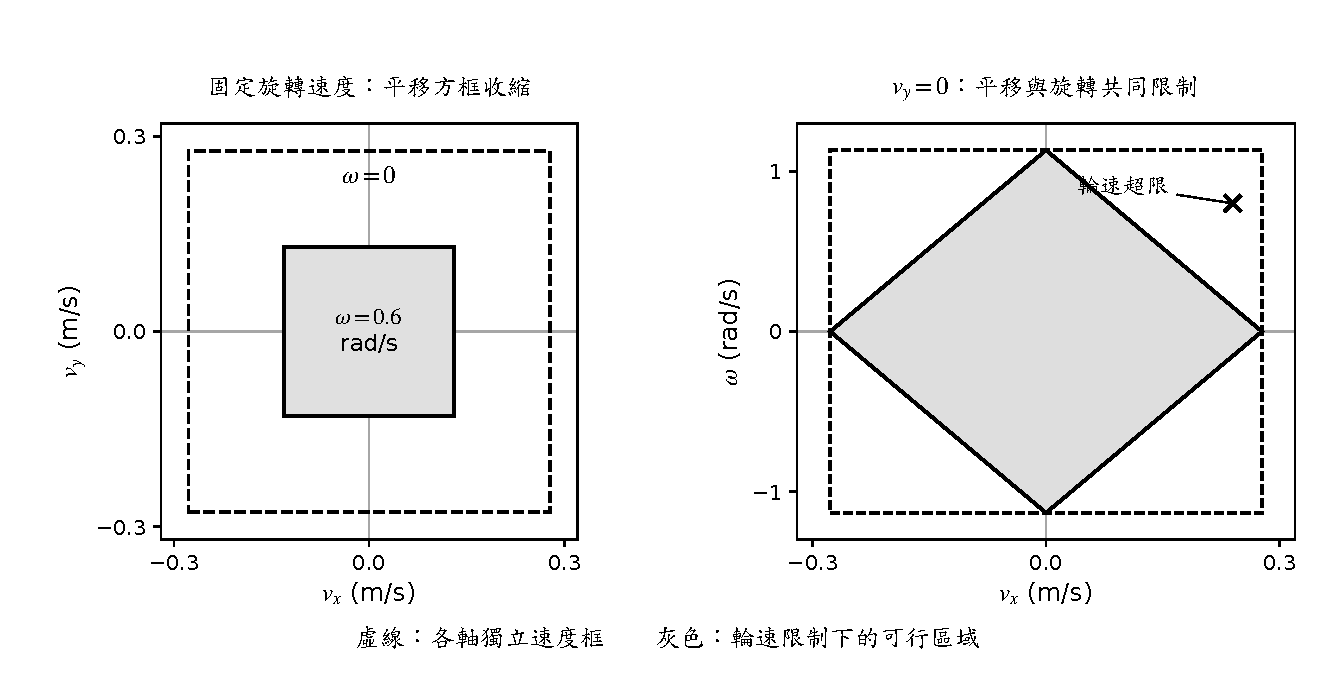
\includegraphics[width=0.98\textwidth]{figsrc/ch03/omni_wheel_velocity_feasible_set.pdf}
    \caption{四輪十字配置之速度可行域：(a) 固定旋轉速度下的 $v_x$--$v_y$ 平移可行域；(b) $v_y=0$ 時的 $v_x$--$\omega$ 剖面。虛線表示各軸獨立速度框，灰色表示輪速限制下的可行區域。}
    \label{fig:ch3_omni_velocity_feasible_set}
\end{figure}

% ==================================================
% 位置：3.3.3
% 正文來源：03_03_objective_constraints.tex
% ==================================================
\begin{figure}[htbp]
    \centering
    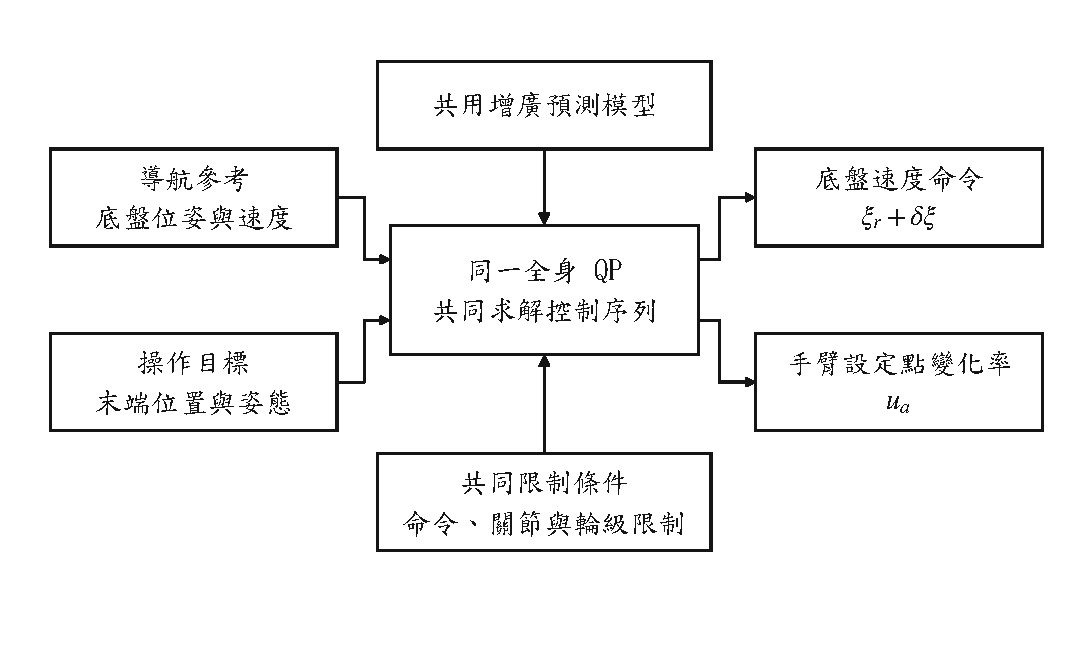
\includegraphics[width=0.98\textwidth]{figsrc/ch03/joint_optimization.pdf}
    \caption{底盤與手臂於同一全身控制問題中共同求解}
    \label{fig:ch3_joint_optimization}
\end{figure}

% ==================================================
% 位置：3.4.1
% 正文來源：03_04_dynamic_obstacle_avoidance.tex
% ==================================================
\begin{figure}[htbp]
    \centering
    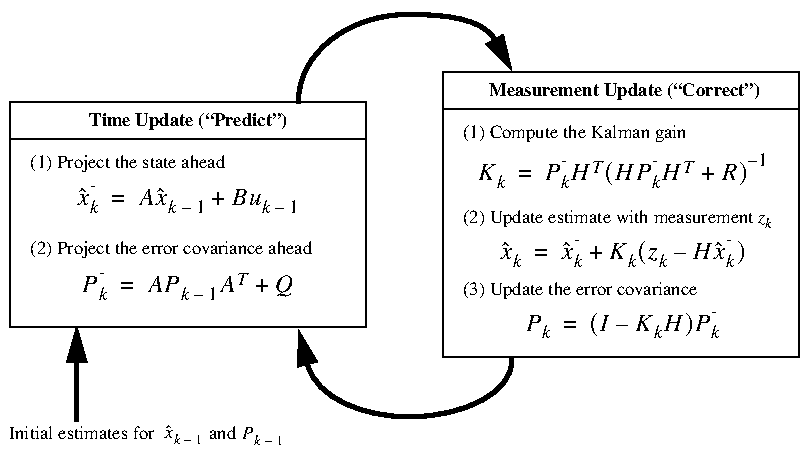
\includegraphics[width=0.98\textwidth]{figsrc/reference_figures/kalman_predict_update_welch2004.pdf}
    \caption{卡爾曼濾波之預測與量測更新流程（引自文獻\cite{welch2004kalman}之圖~1-2）}
    \label{fig:ref_kalman_predict_update}
\end{figure}

% ==================================================
% 位置：3.4.2
% 正文來源：03_04_dynamic_obstacle_avoidance.tex
% ==================================================
\begin{figure}[htbp]
    \centering
    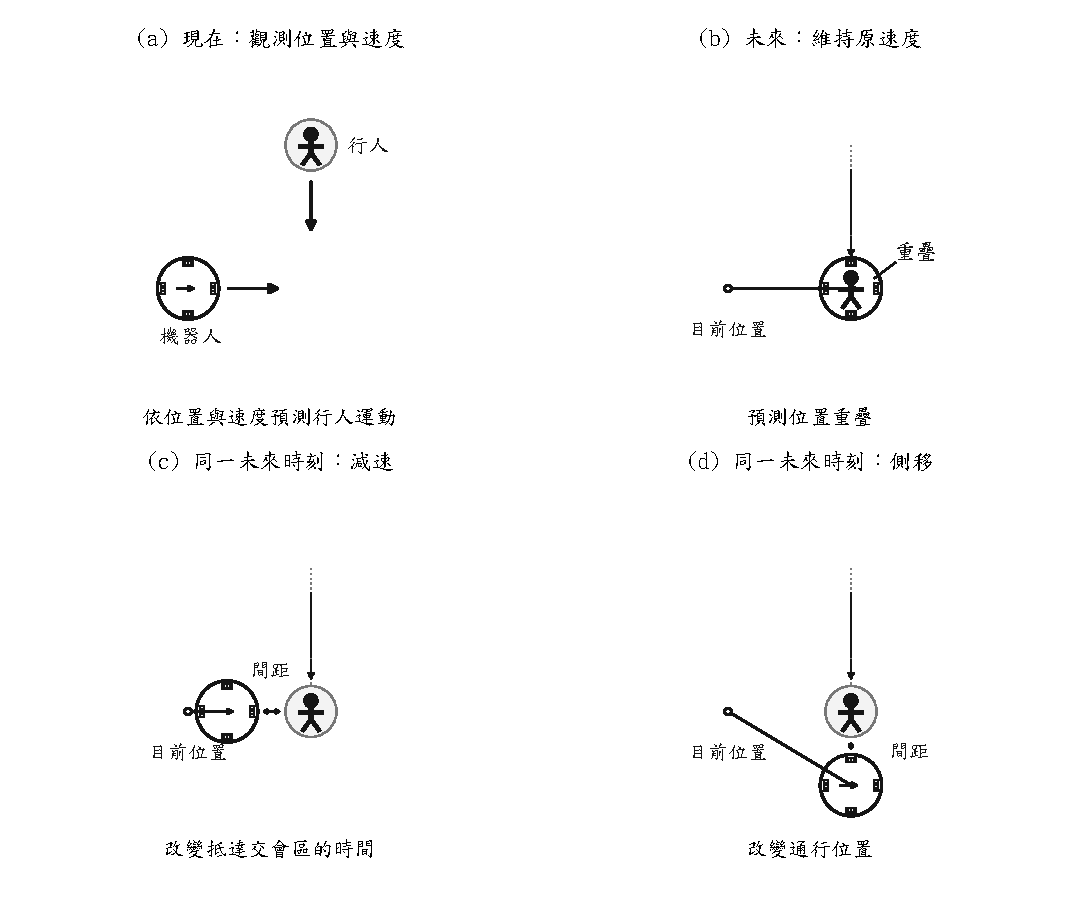
\includegraphics[width=0.98\textwidth]{figsrc/ch03/dynamic_obstacle_prediction.pdf}
    \caption{同一未來時刻下的候選運動比較：(a) 目前觀測；(b) 維持原速度；(c) 降低速度；(d) 側向避讓。}
    \label{fig:ch3_dynamic_obstacle_prediction}
\end{figure}

% ==================================================
% 位置：3.4.5
% 正文來源：03_04_dynamic_obstacle_avoidance.tex
% ==================================================
\begin{figure}[htbp]
    \centering
    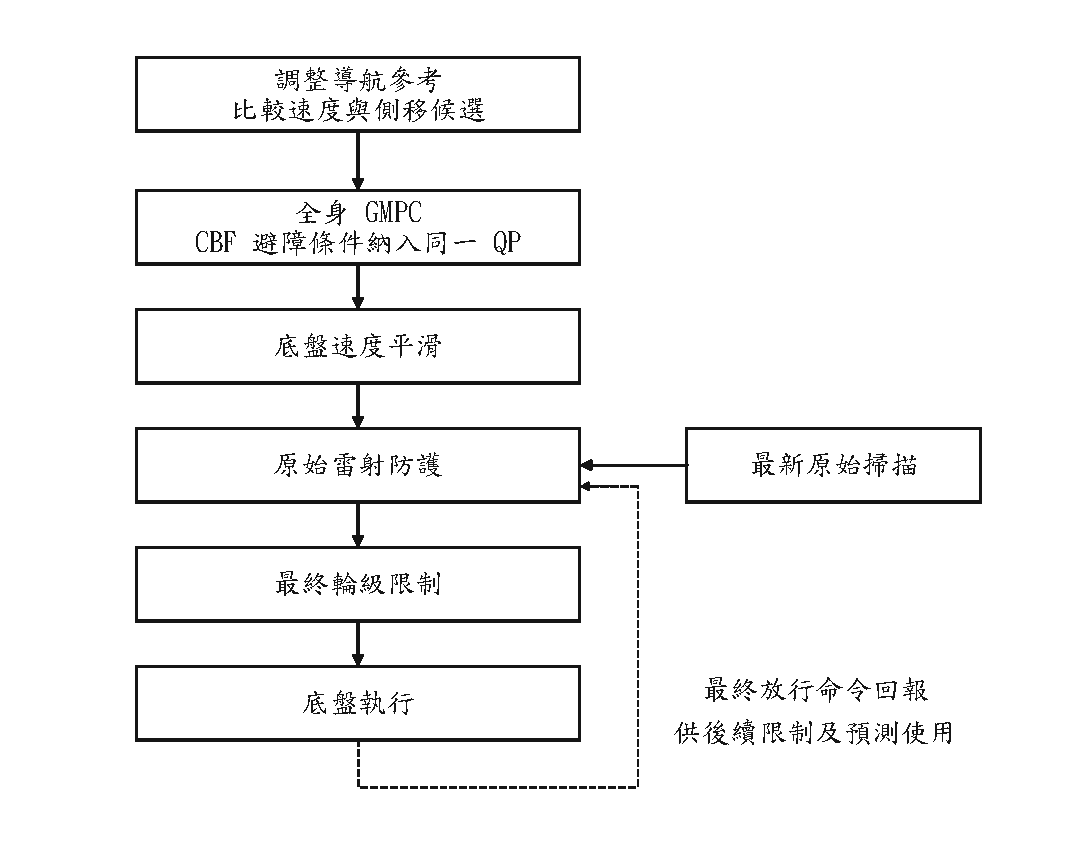
\includegraphics[width=0.98\textwidth]{figsrc/ch03/navigation_command_layers.pdf}
    \caption{導航參考調整、預測避障與底盤命令處理之分層關係}
    \label{fig:ch3_navigation_command_layers}
\end{figure}

% ==================================================
% 位置：3.5.1
% 正文來源：03_05_visual_task_reference.tex
% ==================================================
\begin{figure}[htbp]
    \centering
    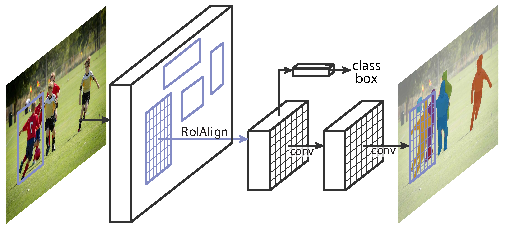
\includegraphics[width=0.95\textwidth]{figsrc/reference_figures/mask_rcnn_framework_he2017.pdf}
    \caption{Mask R-CNN 實例分割方法之原理示意（引自文獻\cite{he2017maskrcnn}之圖~1）}
    \label{fig:ref_mask_rcnn_framework}
\end{figure}

% ==================================================
% 位置：3.5.1
% 正文來源：03_05_visual_task_reference.tex
% ==================================================
\begin{figure}[htbp]
    \centering
    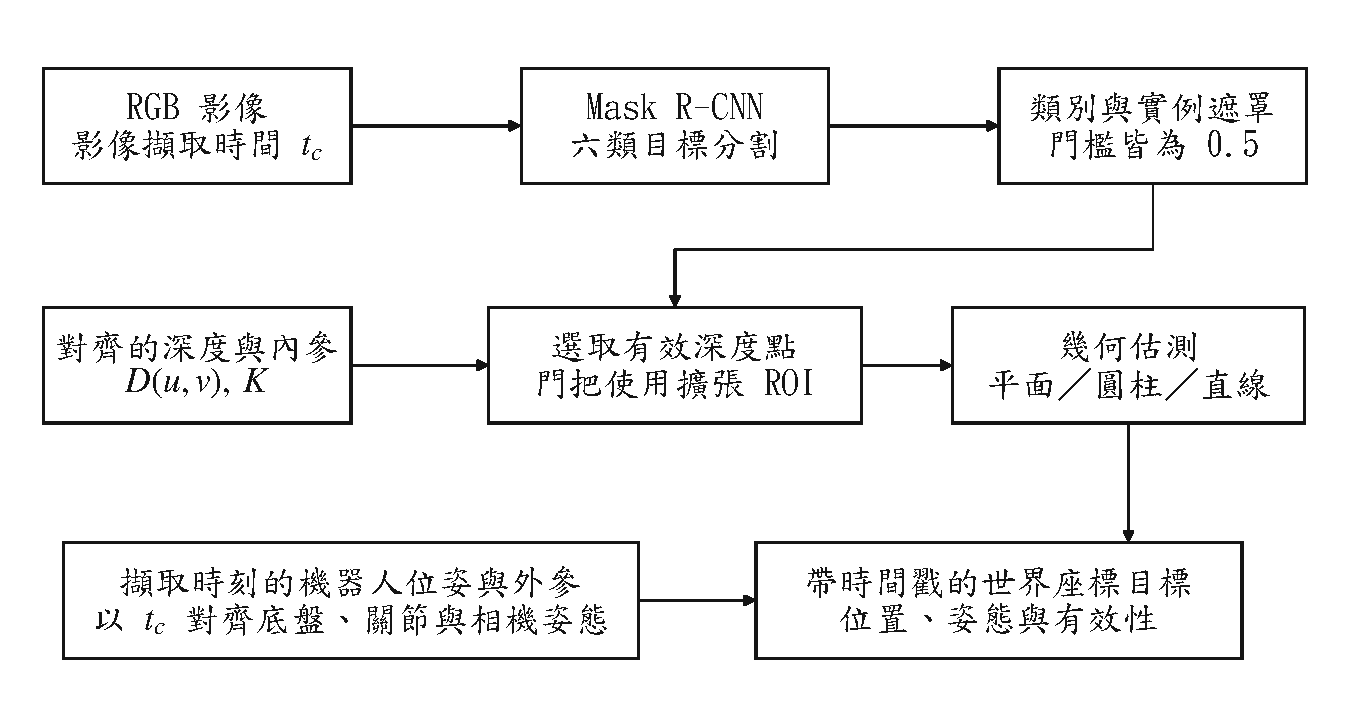
\includegraphics[width=0.98\textwidth]{figsrc/ch03/mask_rcnn_target_pipeline.pdf}
    \caption{本研究之實例分割、深度點選取與帶時間戳操作目標生成流程}
    \label{fig:ch3_mask_rcnn_target_pipeline}
\end{figure}

% ==================================================
% 位置：3.5.2
% 正文來源：03_05_visual_task_reference.tex
% ==================================================
\begin{figure}[htbp]
    \centering
    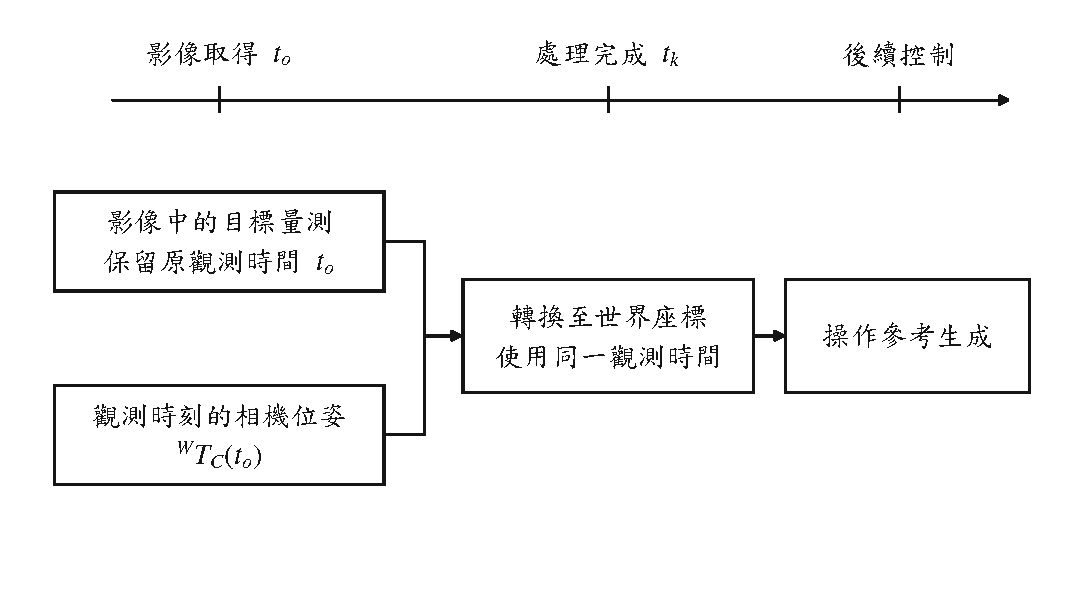
\includegraphics[width=0.98\textwidth]{figsrc/ch03/visual_time_alignment.pdf}
    \caption{視覺量測與相機位姿依觀測時間配對之流程}
    \label{fig:ch3_visual_time_alignment}
\end{figure}

% ==================================================
% 位置：3.5.3
% 正文來源：03_05_visual_task_reference.tex
% ==================================================
\begin{figure}[htbp]
    \centering
    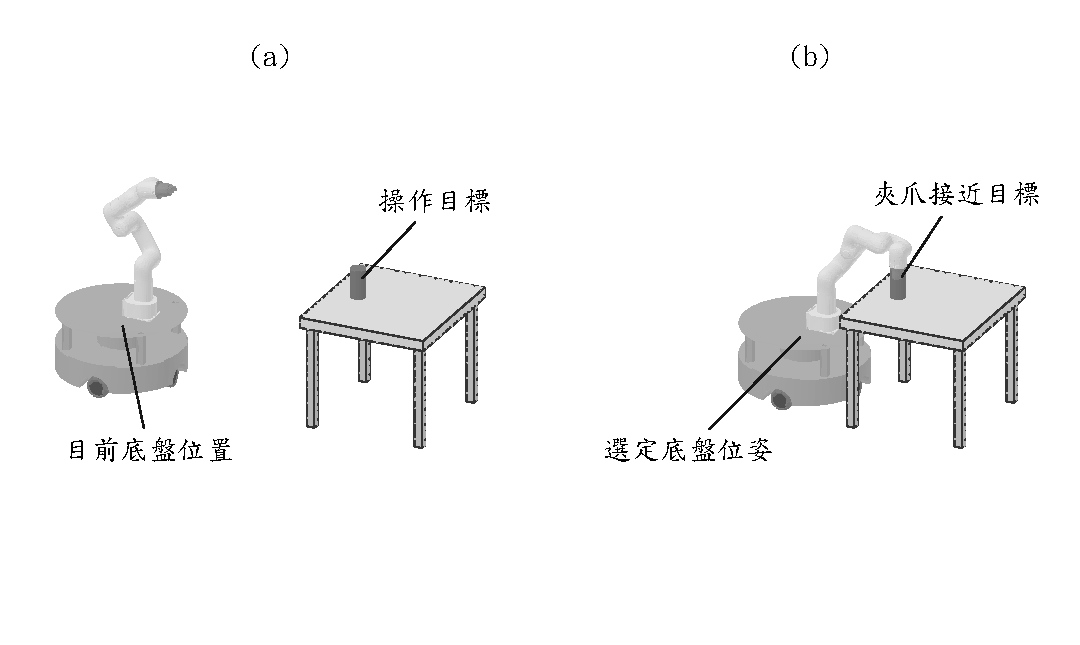
\includegraphics[width=0.98\textwidth]{figsrc/ch03/visual_operation_reference.pdf}
    \caption{操作目標導引之底盤選位：(a) 選位前的機器人與目標位置；(b) 選位後，手臂接近目標。}
    \label{fig:ch3_visual_operation_reference}
\end{figure}

% ==================================================
% 位置：3.5.4
% 正文來源：03_05_visual_task_reference.tex
% ==================================================
\begin{figure}[htbp]
    \centering
    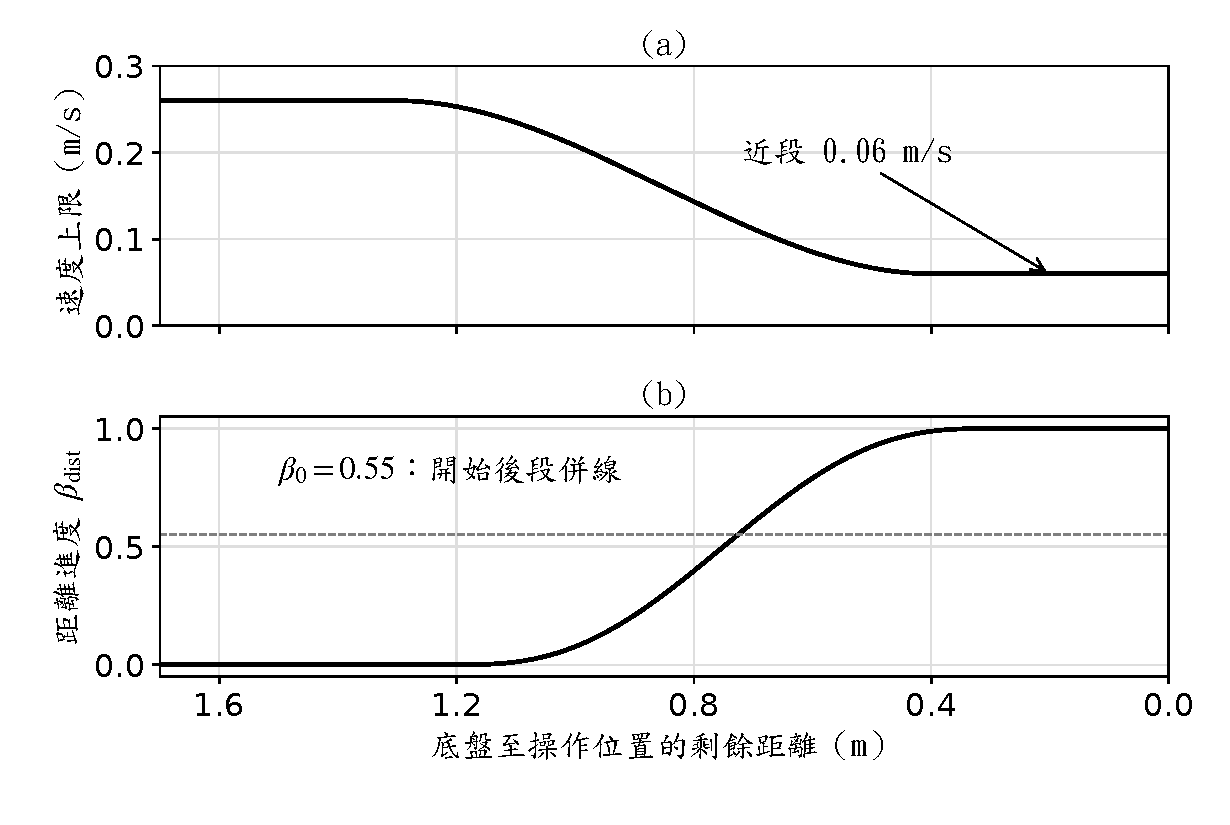
\includegraphics[width=0.98\textwidth]{figsrc/ch03/mobile_approach_distance_profile.pdf}
    \caption{圓柱接近階段之距離規則：(a) 平移逐軸速度上限；(b) 手臂距離展開進度與後段併線門檻。圖中為設計曲線，實際進度另受時間與狀態限制。}
    \label{fig:ch3_mobile_approach_distance_profile}
\end{figure}

% ==================================================
% 位置：3.6.1
% 正文來源：03_06_mobile_constrained_operation.tex
% ==================================================
\begin{figure}[htbp]
    \centering
    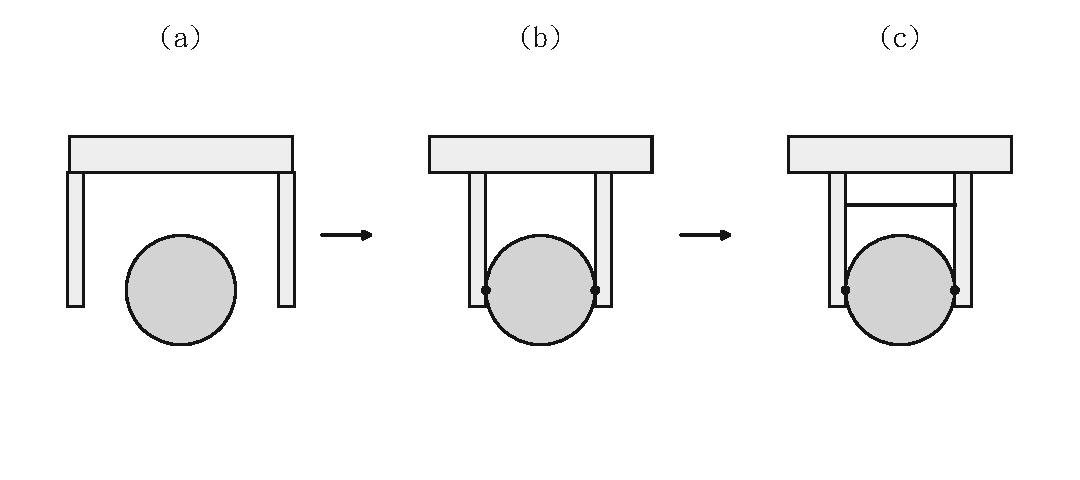
\includegraphics[width=0.98\textwidth]{figsrc/ch03/grasp_state_transition.pdf}
    \caption{抓持狀態之轉移：(a) 張爪接近目標；(b) 閉爪並檢查抓持證據；(c) 證據持續達標且取得必要的連接確認後，進入抓持狀態。}
    \label{fig:ch3_grasp_state_transition}
\end{figure}

% ==================================================
% 位置：3.6.2
% 正文來源：03_06_mobile_constrained_operation.tex
% ==================================================
\begin{figure}[htbp]
    \centering
    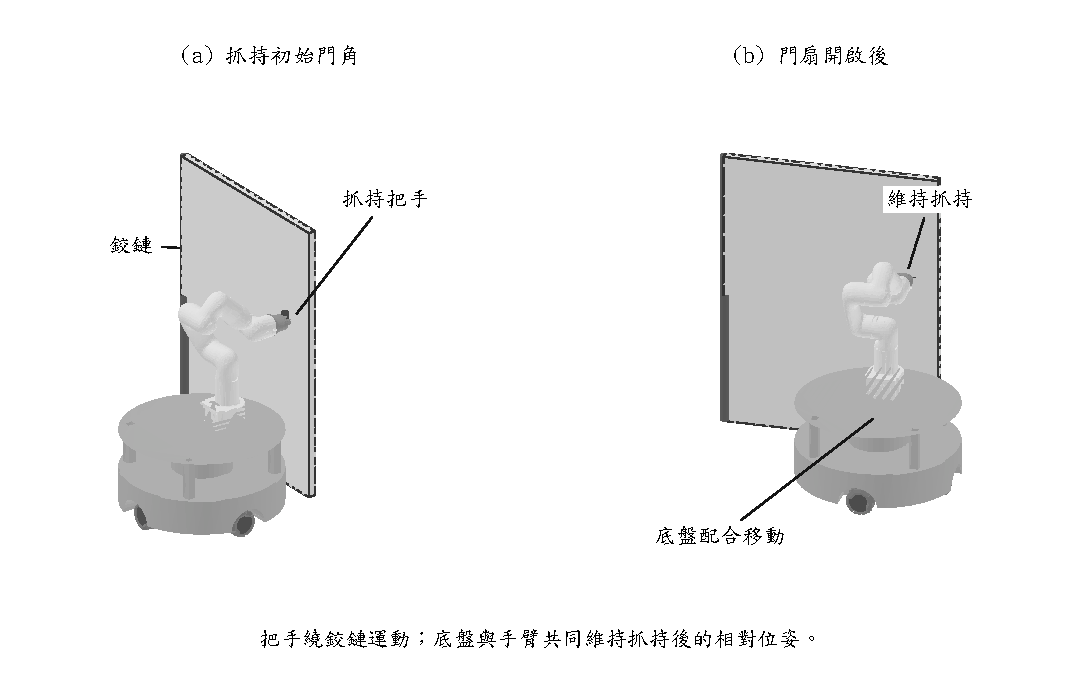
\includegraphics[width=0.98\textwidth]{figsrc/ch03/door_operation_sequence.pdf}
    \caption{門扇操作之全身構型：(a) 抓持初始門角；(b) 門扇開啟後，底盤與手臂配合把手運動。}
    \label{fig:ch3_door_operation_sequence}
\end{figure}

% ==================================================
% 位置：3.6.2
% 正文來源：03_06_mobile_constrained_operation.tex
% ==================================================
\begin{figure}[htbp]
    \centering
    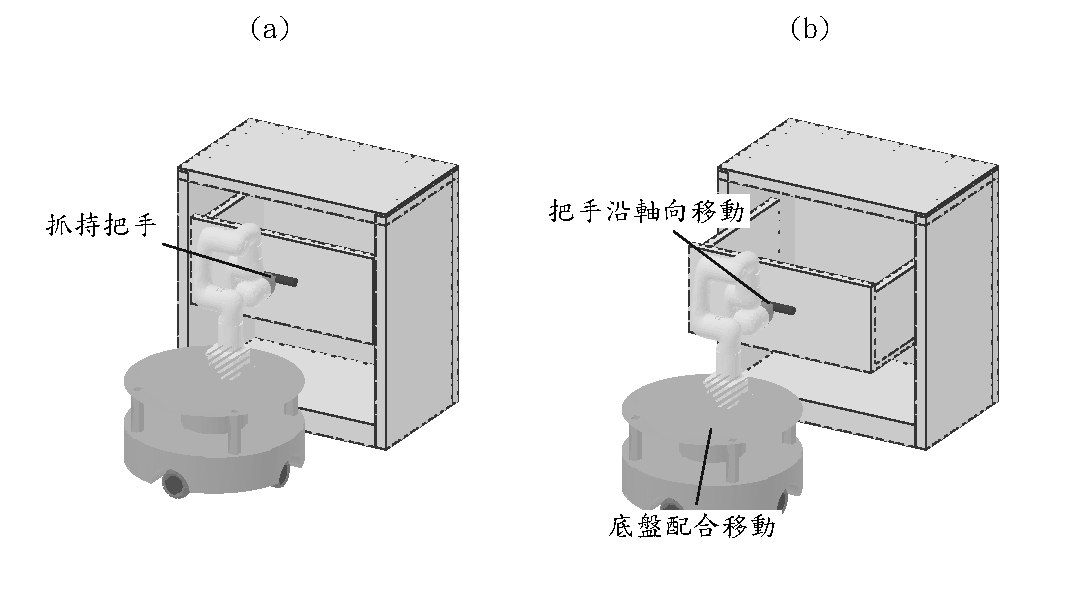
\includegraphics[width=0.98\textwidth]{figsrc/ch03/drawer_operation_sequence.pdf}
    \caption{抽屜操作之全身構型：(a) 抽屜初始位置；(b) 抽屜沿滑軌拉出後，底盤與手臂配合調整。}
    \label{fig:ch3_drawer_operation_sequence}
\end{figure}

% ==================================================
% 位置：3.6.3
% 正文來源：03_06_mobile_constrained_operation.tex
% ==================================================
\begin{figure}[htbp]
    \centering
    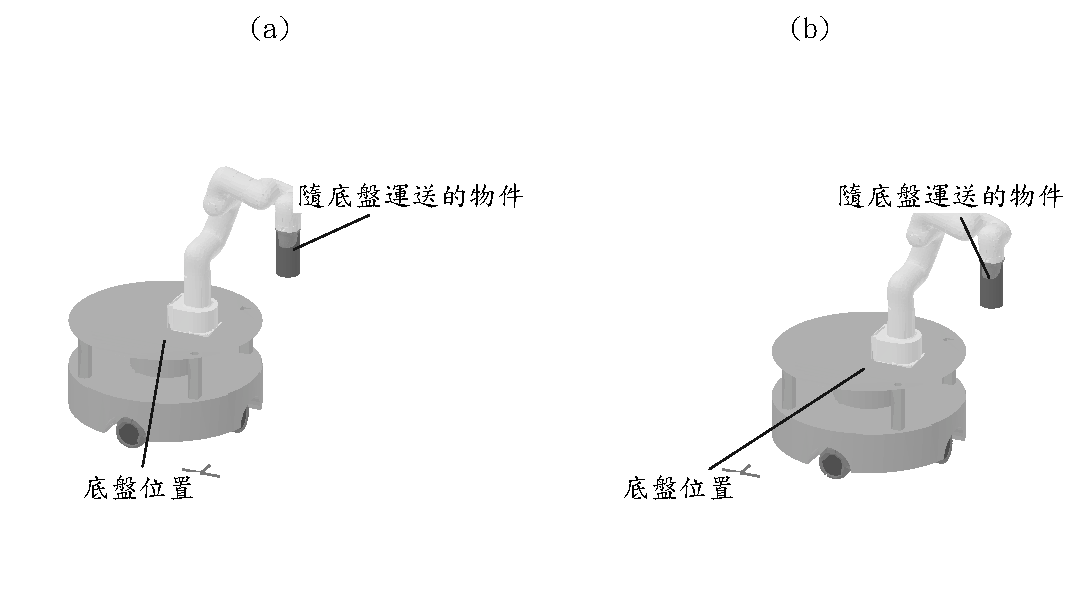
\includegraphics[width=0.98\textwidth]{figsrc/ch03/base_relative_carrying.pdf}
    \caption{相對底盤目標下之持物運送：(a) 底盤移動前；(b) 底盤平移後，維持相同的底盤相對末端構型。}
    \label{fig:ch3_base_relative_carrying}
\end{figure}

% ==================================================
% 位置：3.7.1
% 正文來源：03_07_execution_compensation.tex
% ==================================================
\begin{figure}[htbp]
    \centering
    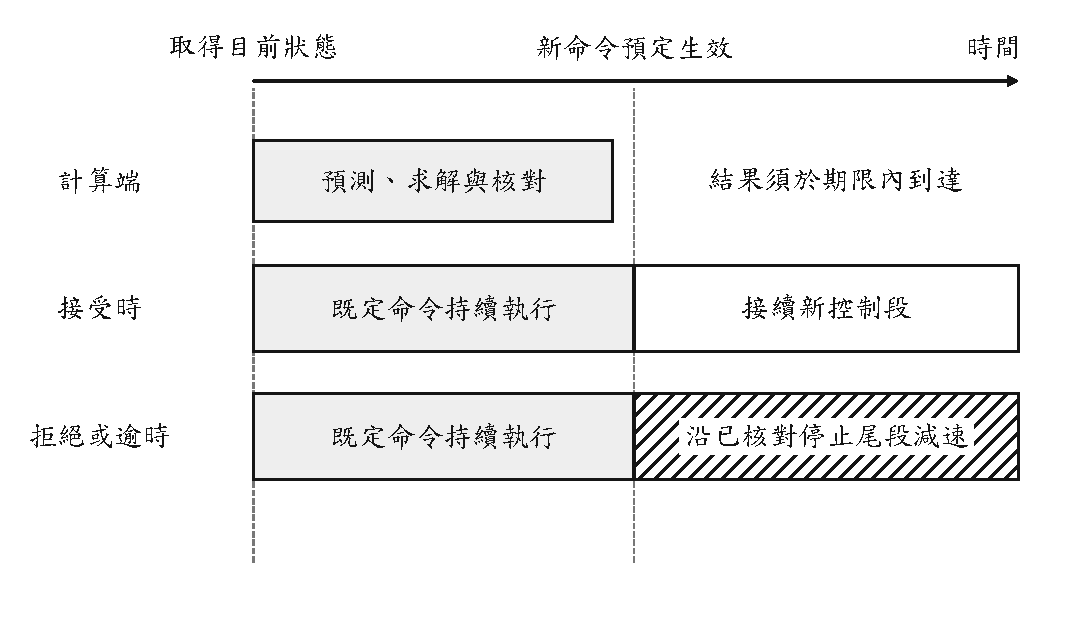
\includegraphics[width=0.98\textwidth]{figsrc/ch03/command_execution_timeline.pdf}
    \caption{控制計算期間之命令接續與停止備援}
    \label{fig:ch3_command_execution_timeline}
\end{figure}

% ==================================================
% 位置：3.7.2
% 正文來源：03_07_execution_compensation.tex
% ==================================================
\begin{figure}[htbp]
    \centering
    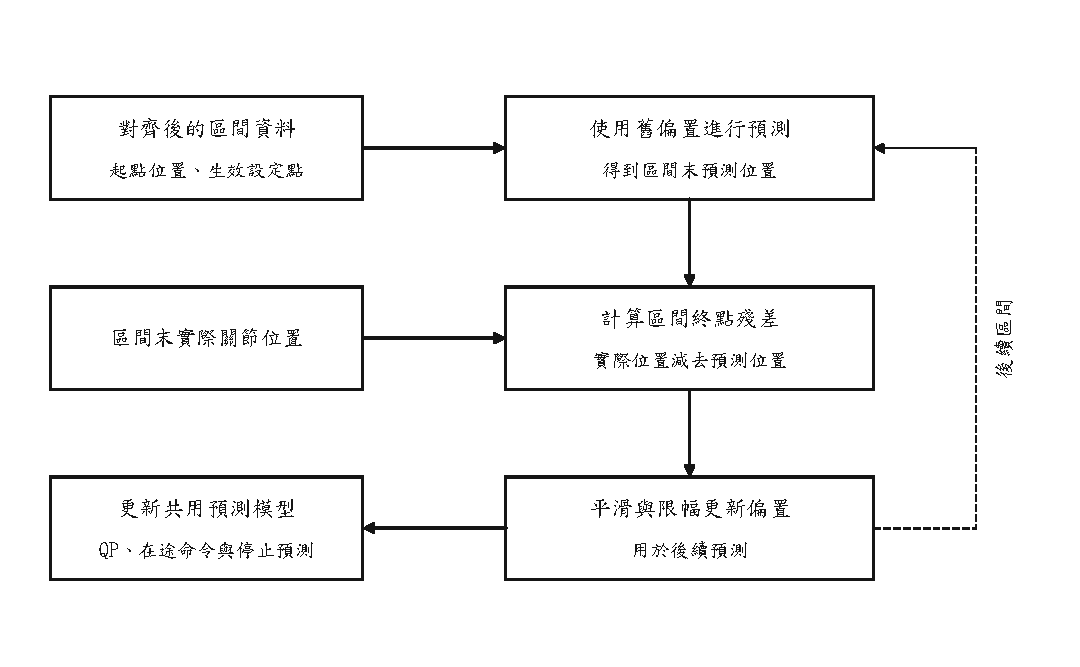
\includegraphics[width=0.98\textwidth]{figsrc/ch03/model_bias_estimation.pdf}
    \caption{模型偏置估測之區間殘差與共用模型更新}
    \label{fig:ch3_model_bias_estimation}
\end{figure}

% ==================================================
% 位置：3.7.2
% 正文來源：03_07_execution_compensation.tex
% ==================================================
\begin{figure}[htbp]
    \centering
    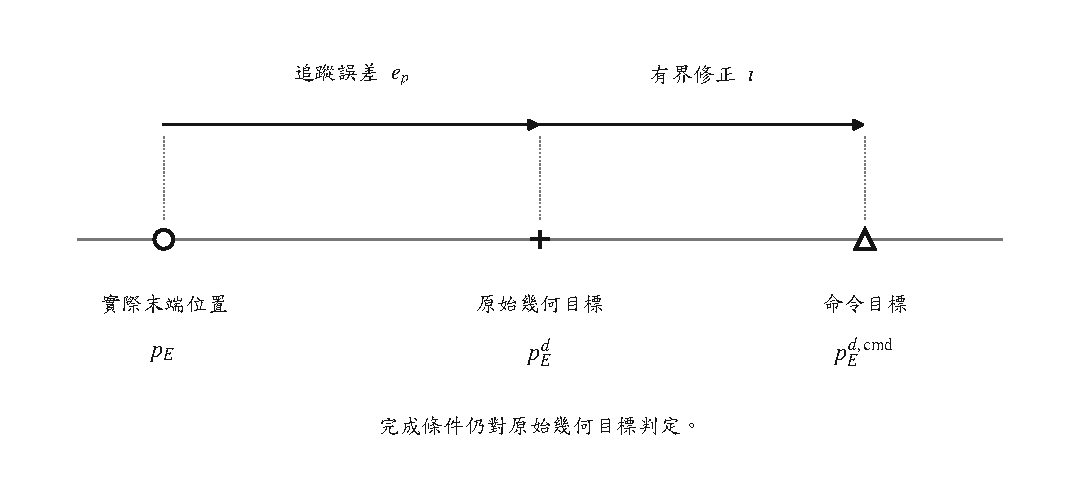
\includegraphics[width=0.98\textwidth]{figsrc/ch03/tcp_target_compensation.pdf}
    \caption{末端原始幾何目標與有界命令目標補償；完成條件依原始幾何目標判定。}
    \label{fig:ch3_tcp_target_compensation}
\end{figure}

% ==================================================
% 位置：3.7.4
% 正文來源：03_07_execution_compensation.tex
% ==================================================
\begin{figure}[htbp]
    \centering
    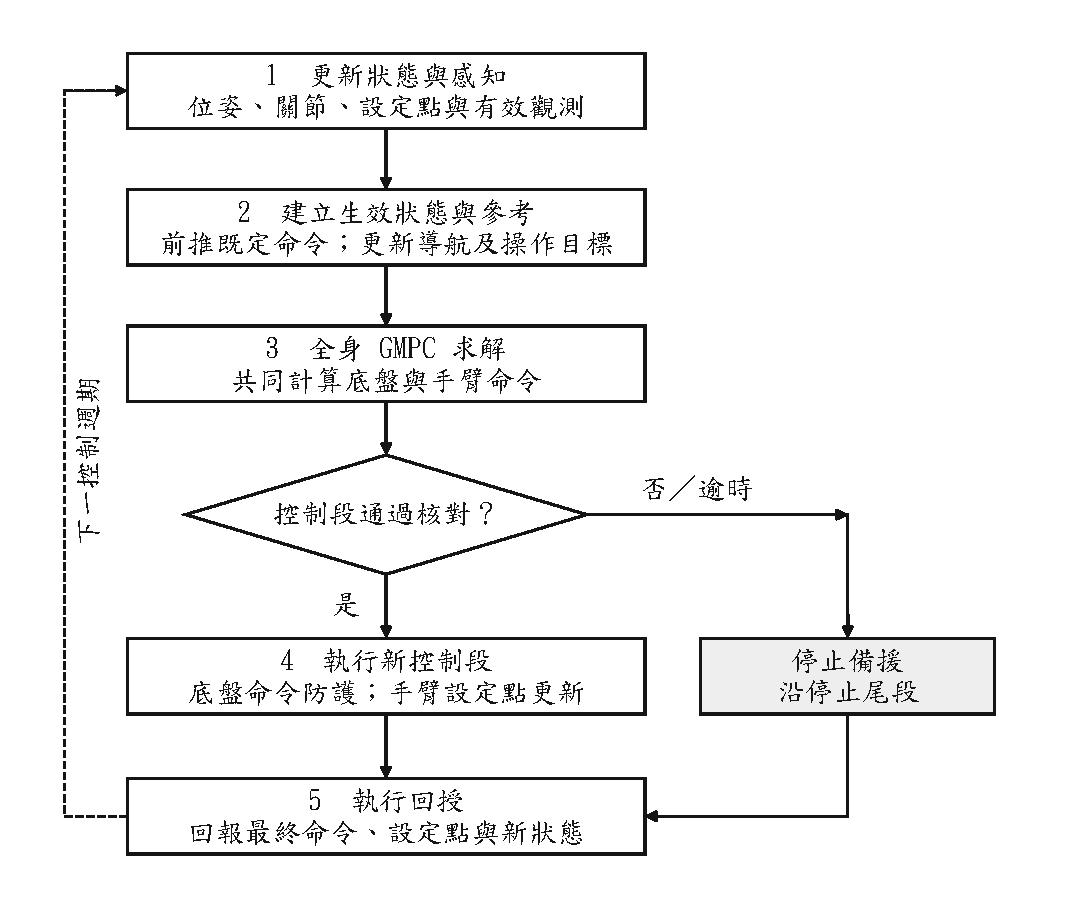
\includegraphics[width=0.98\textwidth]{figsrc/ch03/wholebody_control_workflow.pdf}
    \caption{全身預測控制之計算、命令核對與執行回授流程}
    \label{fig:ch3_wholebody_control_workflow}
\end{figure}

